\begin{exercise}
      {ID-20aedaf3992ebc1b6ba8673186751504895c3c48}
      {Radius}
  \ifproblem\problem\par
    Berechne den Radius des grauen Kreises in Abhängigkeit von $a$.
    \begin{center}
      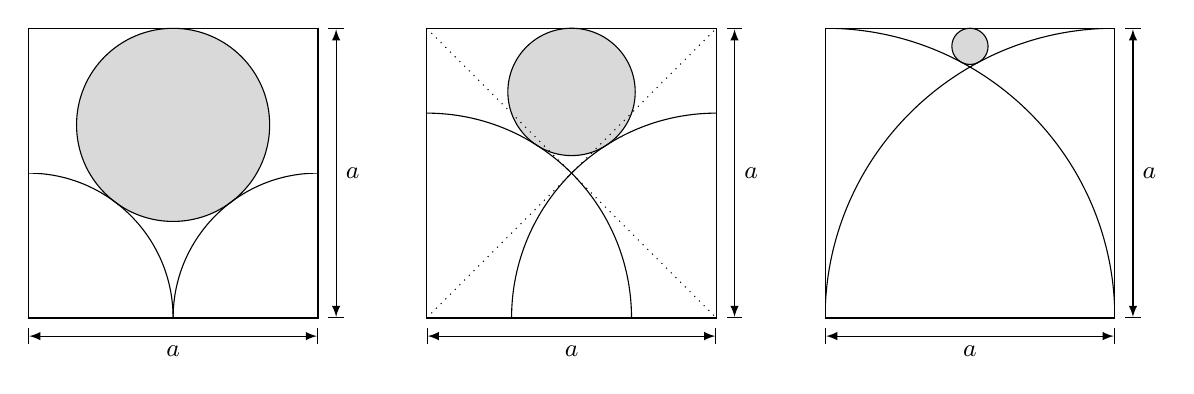
\begin{tikzpicture}[scale=0.92]
        % Figur 1
        \begin{scope}
          % Mittelpunkt des grauen Kreises
          \coordinate (M) at (2, 2.666);
          % Kreisflaeche
          \fill[fill=black!15!white] (M) circle[radius=1.333];
          % Quadrat
          \draw (0, 0) rectangle (4, 4);
          % Kreis
          \draw (M) circle[radius=1.333];
          % Viertelkreise
          \begin{scope}
            \clip (0, 0) rectangle (4, 2);
            \draw (0, 0) circle[radius=2];
            \draw (4, 0) circle[radius=2];
          \end{scope}
          % Bezeichnung
          \draw[|<->|, >=latex, shift={(0, -0.25)}] (0, 0) -- node[below] {{\small$a$}} (4, 0);
          \draw[|<->|, >=latex, shift={(0.25, 0)}] (4, 0) -- node[right] {{\small$a$}} (4, 4);
        \end{scope}
        % Figur 2
        \begin{scope}[xshift=5.5cm]
          % Mittelpunkt des grauen Kreises
          \coordinate (M) at (2, 3.121);
          % Kreisflaeche
          \fill[fill=black!15!white] (M) circle[radius=0.879];
          % Quadrat
          \draw (0, 0) rectangle (4, 4);
          % Diagonalen
          \draw[style=dotted] (0, 0) -- (4, 4);
          \draw[style=dotted] (0, 4) -- (4, 0);
          % Kreis
          \draw (M) circle[radius=0.879];
          % Kreise
          \begin{scope}
            \clip (0, 0) rectangle (4, 4);
            \draw (0, 0) circle[radius=2.828];
            \draw (4, 0) circle[radius=2.828];
          \end{scope}
          % Bezeichnung
          \draw[|<->|, >=latex, shift={(0, -0.25)}] (0, 0) -- node[below] {{\small$a$}} (4, 0);
          \draw[|<->|, >=latex, shift={(0.25, 0)}] (4, 0) -- node[right] {{\small$a$}} (4, 4);
        \end{scope}
        % Figur 3
        \begin{scope}[xshift=11cm]
          % Mittelpunkt des grauen Kreises
          \coordinate (M) at (2, 3.75);
          % Kreisflaeche
          \fill[fill=black!15!white] (M) circle[radius=0.25];
          % Quadrat
          \draw (0, 0) rectangle (4, 4);
          % Kreis
          \draw (M) circle[radius=0.25];
          % Kreise
          \begin{scope}
            \clip (0, 0) rectangle (4, 4);
            \draw (0, 0) circle[radius=4];
            \draw (4, 0) circle[radius=4];
          \end{scope}
          % Bezeichnung
          \draw[|<->|, >=latex, shift={(0, -0.25)}] (0, 0) -- node[below] {{\small$a$}} (4, 0);
          \draw[|<->|, >=latex, shift={(0.25, 0)}] (4, 0) -- node[right] {{\small$a$}} (4, 4);
        \end{scope}
      \end{tikzpicture}
    \end{center}
  \fi
  \ifoutline\outline\par
    Über den \emph{Satz des Pythagoras} lässt sich jeweils ein Zusammenhang
    zwischen $a$ und $r$ herstellen:
    \begin{center}
      % Figur 1
      \begin{tikzpicture}[scale=0.92]
        % Mittelpunkt des grauen Kreises
        \coordinate (M) at (2, 2.666);
        % Kreisflaeche
        \fill[fill=black!15!white] (M) circle[radius=1.333];
        % Quadrat
        \draw (0, 0) rectangle (4, 4);
        % Kreis
        \draw (M) circle[radius=1.333];
        % Viertelkreise
        \begin{scope}
          \clip (0, 0) rectangle (4, 2);
          \draw (0, 0) circle[radius=2];
          \draw (4, 0) circle[radius=2];
        \end{scope}
        % Mittelpunkt des Kreises
        \fill (M) circle[radius=0.75pt];
        % Beschriftung: Ri
        \path (0, 0) -- node[right]{{\small$R_{i}$}}($(0, 0)!2cm!0:(M)$);
        % Beschriftung: r
        \path (M) -- node[left]{{\small$r_{i}$}}($(M)!1.333cm!0:(0, 0)$);
        % rechtwinkliges Dreieck
        \draw (M) -- (0, 0) -- (2, 0) -- cycle;
        % Seiten des Quadrats
        \draw[|<->|, >=latex, shift={(0, -0.25)}] (0, 0) -- node[below] {{\small$a$}} (4, 0);
        \draw[|<->|, >=latex, shift={(0.25, 0)}] (4, 0) -- node[right] {{\small$a$}} (4, 4);
        % Ansatz
        \node[right] at (6, 2)
        {%
          \begin{minipage}{8cm}
            \setlength{\abovedisplayskip}{0pt}%
            \begin{equation*}
              \begin{split}
                (R_{i}+r_{i})^2&=\left(\frac{a}{2}\right)^2+(a-r_{i})^2\\[2ex]
                R_{1}=\frac{a}{2}
                \qquad
                R_{2}&=\frac{\sqrt{2}}{2}\cdot a
                \qquad
                R_{3}=a
              \end{split}
            \end{equation*}
          \end{minipage}%
        };
      \end{tikzpicture}
    \end{center}
  \fi
  \ifoutcome\outcome\par
    \newcommand{\fakewidth}[1]
    {%
      \makebox[0pt][l]
      {%
        \ensuremath
        {%
          \displaystyle#1%
        }%
      }%
    }%

    Für den Radius des grauen Kreises in der linken Zeichnung gilt:
    \begin{alignat*}{3}
                     &\qquad & \left(\frac{a}{2}+r\right)^2&=\left(\frac{a}{2}\right)^2+(a-r)^2 & \qquad&                          \\[2ex]
      \Leftrightarrow&\qquad &         \frac{a^2}{4}+ar+r^2&=\frac{a^2}{4}+a^2-2ar+r^2          & \qquad&|-\frac{a^2}{4}\quad|-r^2 \\[2ex]
      \Leftrightarrow&\qquad &                       ar    &=              a^2-2ar              & \qquad&|+2ar                     \\[2ex]
      \Leftrightarrow&\qquad &                      3ar    &=              a^2                  & \qquad&|:(3a)                    \\[2ex]
      \Leftrightarrow&\qquad &                        r    &=        \frac{a}{3}                & \qquad&
    \end{alignat*}

    Für den Radius des grauen Kreises in der mittleren Zeichnung gilt:
    \begin{alignat*}{3}
                     &\qquad & \left(\frac{\sqrt{2}}{2}\cdot a+r\right)^2   &=\left(\frac{a}{2}\right)^2+(a-r)^2  & \qquad&                                  \\[2ex]
      \Leftrightarrow&\qquad &               \frac{a^2}{2}+\sqrt{2}ar+r^2   &=\frac{ a^2}{4}+a^2-2ar+r^2          & \qquad&|-r^2                             \\[2ex]
      \Leftrightarrow&\qquad &               \frac{a^2}{2}+\sqrt{2}ar       &=\frac{5a^2}{4}    -2ar              & \qquad&|+2ar\quad|-\frac{a^2}{2}         \\[2ex]
      \Leftrightarrow&\qquad &                             \sqrt{2}ar+2ar   &=\frac{5a^2}{4}-\frac{a^2}{2}        & \qquad&                                  \\[2ex]
      \Leftrightarrow&\qquad &                     ar\left(\sqrt{2}+2\right)&=\frac{3a^2}{4}                      & \qquad&|:a\quad|:\left(\sqrt{2}+2\right) \\[2ex]
      \Leftrightarrow&\qquad &                      r                       &=\frac{3a}{4\left(\sqrt{2}+2\right)}
                                                                             =\fakewidth{\frac{3a}{\sqrt{32}+8}}  & \qquad&
    \end{alignat*}

    Für den Radius des grauen Kreises in der rechten Zeichnung gilt:
    \begin{alignat*}{3}
                     &\qquad & (a+r)^2     &=\left(\frac{a}{2}\right)^2+(a-r)^2 & \qquad&                \\[2ex]
      \Leftrightarrow&\qquad & a^2+2ar+r^2 &=\frac{a^2}{4}+a^2-2ar+r^2          & \qquad&|-a^2\quad|-r^2 \\[2ex]
      \Leftrightarrow&\qquad &     2ar     &=\frac{a^2}{4}    -2ar              & \qquad&|+2ar           \\[2ex]
      \Leftrightarrow&\qquad &     4ar     &=\frac{a^2}{4}                      & \qquad&|:(4a)          \\[2ex]
      \Leftrightarrow&\qquad &       r     &=\frac{a}{16}                       & \qquad&
    \end{alignat*}
  \fi
\end{exercise}
